\documentclass[border=10pt]{standalone}

\usepackage{tikz}
\usepackage{tikzsymbols}
\usetikzlibrary{calc,patterns,shapes.geometric}

\def\centerarc[#1](#2)(#3:#4:#5){\draw[#1] ($(#2)+({#5*cos(#3)},{#5*sin(#3)})$) arc (#3:#4:#5);}

\begin{document}
	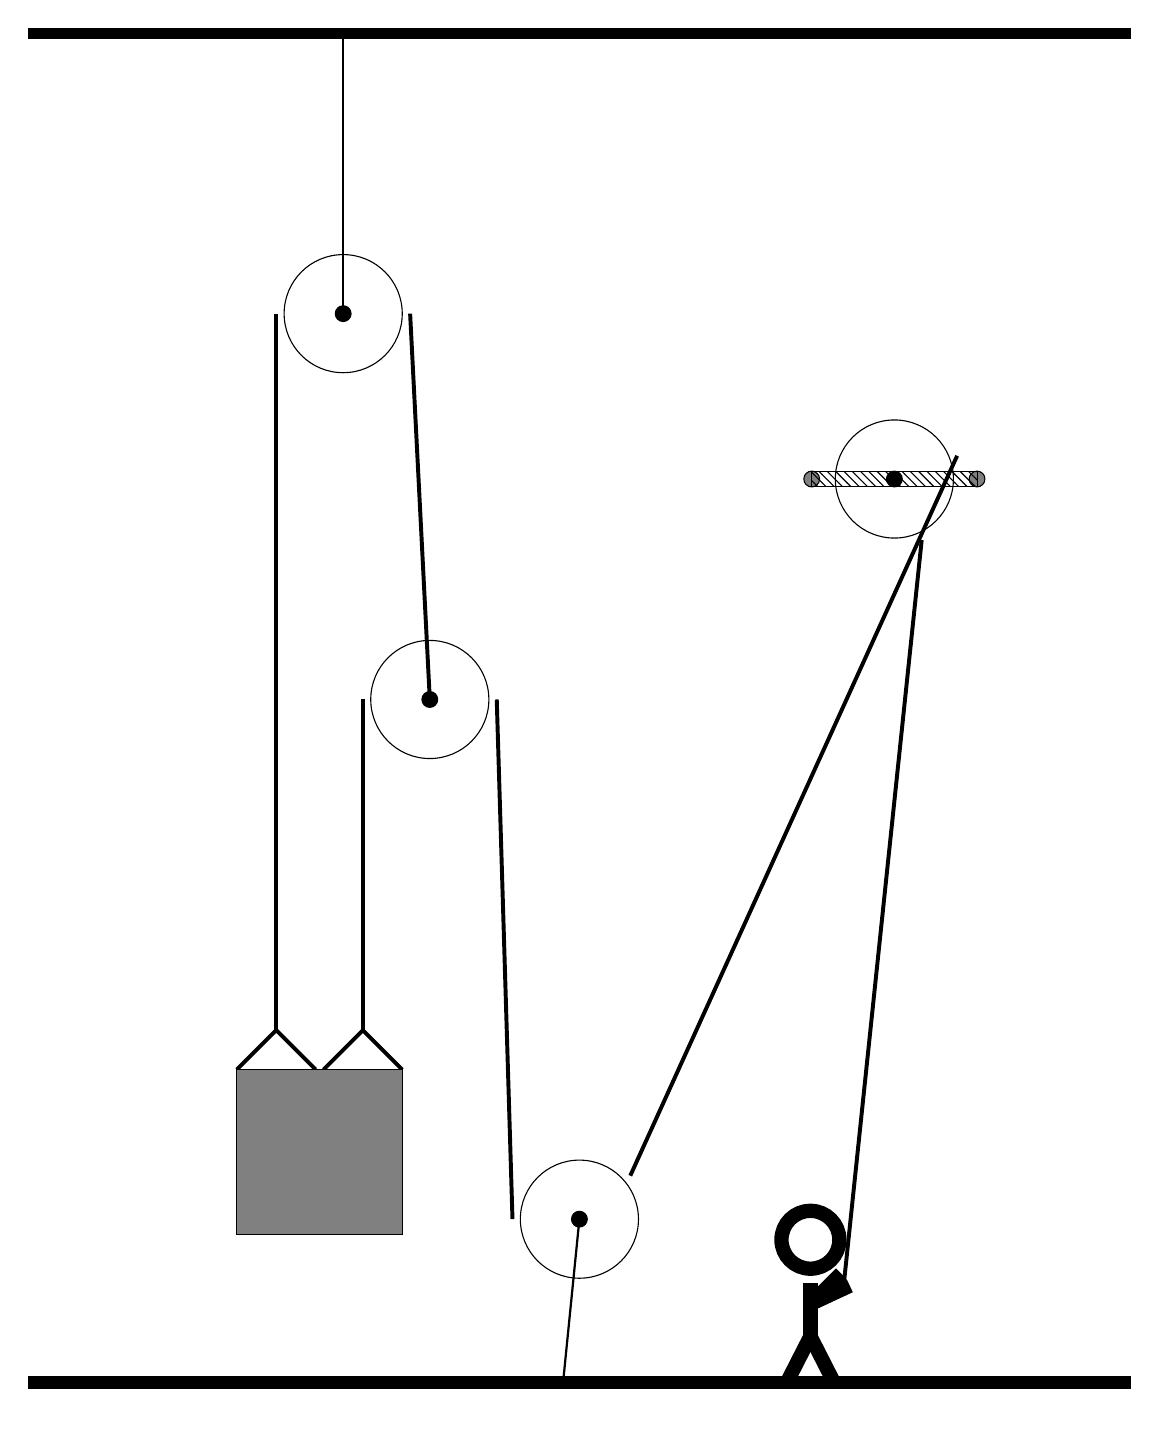
\begin{tikzpicture}
		%%%%% START %%%%%
		\draw[fill=black] (-2, 14) rectangle (12, 14.125);
		
		\draw (2, 10.5) circle (0.75);
		\draw[fill=black] (2, 10.5) circle (0.1);
		\draw[thick] (2, 10.5) -- (2, 14);
		
		\draw (3.1, 5.6) circle (0.75);
		\draw[fill=black] (3.1, 5.6) circle (0.1);
		
		\draw (5, -1) circle (0.75);
		\draw[fill=black] (5, -1) circle (0.1);
		\draw[thick] (5, -1) -- (4.8, -3);
		
		\draw (9, 8.4) circle (0.75);
		\draw[fill=black] (9, 8.4) circle (0.1);
		\draw[fill=black!50] (7.95, 8.4) circle (0.1);
		\draw[fill=black!50] (10.05, 8.4) circle (0.1);
		\draw[pattern=north west lines, pattern color=black] (7.95, 8.5) rectangle (10.05, 8.3);
		
		\draw[line width = 0.5mm]  (0.65, 0.9) -- (1.15, 1.4) -- (1.65, 0.9);
		\draw[line width = 0.5mm]  (1.75, 0.9) -- (2.25, 1.4) -- (2.75, 0.9);
		\draw[fill=black!50] (0.65, 0.9) rectangle (2.75, -1.2);
		
		\draw[line width = 0.5mm] (1.15, 10.5) -- (1.15, 1.4);
		\centerarc[line width = 0.5mm](2, 10.5)(0:180:0.85);
		\draw[line width = 0.5mm] (2.85, 10.5) -- (3.1, 5.6);
		\draw[line width = 0.5mm] (2.25, 5.6) -- (2.25, 1.4);
		\centerarc[line width = 0.5mm](3.1, 5.6)(0:180:0.85);
		\draw[line width = 0.5mm] (3.95, 5.6) -- (4.15, -1);
		\centerarc[line width = 0.5mm](5, -1)(180:340:0.85);
		\draw[line width=0.5mm](5.646, -0.448) -- (9.797, 8.695);
		\centerarc[line width = 0.5mm](9, 8.4)(-20:170:0.85);
		\draw[line width=0.5mm](9.347, 7.624) --  (8.35, -1.9);
		
		\node at (8, -2) {\Strichmaxerl[10][225][25]};
		
		\draw[fill=black] (-2, -3) rectangle (12, -3.15);
		%%%%% END %%%%%
	\end{tikzpicture}
\end{document}